This chapter is a continuation of the literature review, however, three theoretical approaches to place-centred design is presented; Hybrid Place, Place as a dialogue, and, Sense-making. These approaches have all directly guided fieldwork and analysis-oriented efforts, and as you will come to see in Chapter 4, we build upon and borrow concepts from all three approaches to build a theoretical framework that can help both identify and analyse dialogical relations in a museum space.

\subsubsection{Technologically-enhanced physical spaces}
The perspective of “Ubiquitous Computing,” proposed in the early 1990s by Mark Weiser, is based on technological developments that make it possible to embed powerful computational elements and digital components into everyday objects, portable devices, and the built environment \autocite[p. 217]{ciolfi_space_2005}. This trend is inducing significant changes not only in the development and implementation of new technology but also, and more interestingly, in the relationship between interactive systems and their users \autocite[p. 217]{ciolfi_space_2005}. Design must now concern itself with the physical environments people experience in their daily lives. People will encounter technologically enhanced spaces and artefacts as they move through a variety of environments \autocite[p. 217]{ciolfi_space_2005}. These systems will change how physical spaces are used and shaped by people, where the systems can react and respond to their presence and actions. The activities of interacting with the space and its elements and interacting with the computer system will merge into each other \autocite[p. 217]{ciolfi_space_2005}.

The Interaction Design (IxD) field is currently enduring a shift in the understanding of the relationship between people and technologies, where HCI primarily has focused on a single user's traits and preferences, a one-to-one relationship with the computer system \autocite[p. 217]{ciolfi_space_2005}. As a result, interaction Design is now more than ever concerned with the social, emotional, and contextual factors influencing human interaction with a computer system \autocite[p. 217]{ciolfi_space_2005}. Context-aware systems are those that can sense features of the physical setting and feed a representation of this data into the system itself. The sensing devices can be located both around the physical environment and on the bodies of the inhabitants \autocite[p. 218]{ciolfi_space_2005}.

Ciolfi and Bannon's research aim to apply the concept of a place to a particular set of ubiquitous systems: technologically-enhanced physical spaces. With ubiquitous technologies becoming more reliable and widespread, we are now dealing with fully interactive physical spaces containing tangible elements acting as interfaces to access features of the digital domain. The way this is applied and understood in this thesis, the concept of place can assist interaction designers in understanding interaction dynamics in this context. This way, one can aim to propose practical design concepts: "where place goes beyond the vision of space just as a physical setting, a container, and includes many dimensions of human experience within an environment" \autocite[p. 221]{ciolfi_space_2005}.


% Illustration of Hybrid Place?
\break
\section{Hybrid Place}
This section presents the Hybrid Place approach. As the thesis unfolds, I will often refer to this approach as it is; either \emph{the Hybrid Place approach} or simply \emph{Hybrid Place}. This is a place-centered approach to how geographical notions of space and place can aid designers in creating meaningful interactions between end-users and technologically augmented physical spaces. This is aided through four dimensions, presented in section 3.1.2. The four dimensions have both a formative application for the design of the data-gathering guides, as evident in the Appendix, the Design Process (Chapter 6), and Chapter 4: A new way of designing for meaningfulness.

\subsection{Designing a hybrid place}
"Thanks to the development of ubiquitous and pervasive technologies, research focusing on the design of novel interactive artefacts has recently become more concerned with studying and understanding the spatial properties of the world" \autocite[p. 159]{hybridplace_ciolfi}. "Bringing technologies beyond the desktop and into the world requires an ever-increasing interest in the \emph{physical environment} where interaction occurs" \autocite[p. 159]{hybridplace_ciolfi}. "Designing the interaction between ubiquitous technologies and users involves both a re-conceptualization of the interface as an assembly of tangible physical elements (including furniture and everyday objects) and, importantly, an understanding of the relationship between users and the physical space that is augmented by the technology" \autocite[p. 159]{hybridplace_ciolfi}. Following the interest in the physical environment where interaction occurs, Ciolfi and Bannon discuss how geographical notions of space and place can aid designers in creating meaningful interactions between end-users and technologically augmented physical spaces. After reviewing literature discussing the use of spatial concepts and metaphors within the interaction design field, they present a conceptual framework to design technologically enhanced environments for museums and exhibitions. Their goal is to show how a place-centered approach can practically guide and support design, specifically within a setting that has seen many cases of technology introduction that have led to the visitors' distraction from the museum holdings instead of extending and supporting the museum experience \autocite[p. 159-160]{hybridplace_ciolfi}.


Ciolfi and Bannon (2007) are particularly interested in the experience of place. They strive to understand the ways people come to ascribe meanings to particular places and how certain places evoke complex webs of significance for people \autocite[p. 160]{hybridplace_ciolfi}. This is different from other similar research approaches that have attempted to use ideas from architecture and urban planning to inform the placement of interactive artefacts, e.g., \autocite{Cullen_book}, or noting how the environment affects people's movement and interaction, e.g., \autocite{Alexander_book}. Instead, they base their articulation of place on the work of the geographer \autocite{Tuan_book}. According to Tuan, it is only natural that a place is grounded in the physical, material reality of the world. And that experience is shaped through physical sensing, exploration, and habitation. Based on Tuan's conceptualizations, Ciolfi and Bannon propose an articulation of the concept of place that highlight the different dimensions as interconnected aspects of the individual experience, see Figure 3.1:

\begin{figure}[H]
\centering 
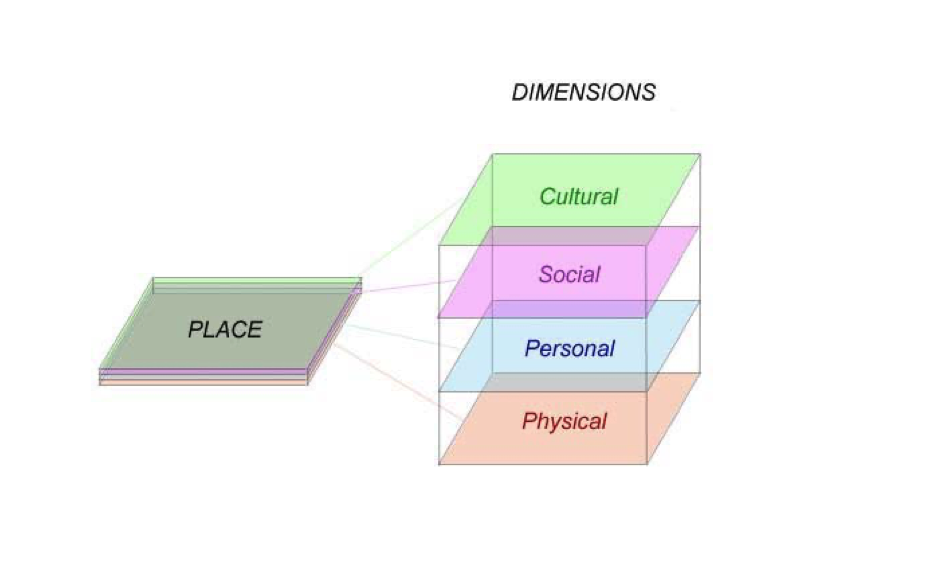
\includegraphics[width=12.5cm]{pictures/Theory/tuans_dimensions.png}
\caption{Tuan's conceptualization of place}
\autocite[p. 224]{ciolfi_space_2005}
\centering
\end{figure}

The articulation of the four dimensions of place can help interaction design in interactive spaces by bringing aspects of individual traits and preferences, social interaction, and cultural influences together with the physical features of the space \autocite[p. 163]{hybridplace_ciolfi}. "These dimensions do not exist \emph{a priori}, but emerge and become visible in practice and experience as they lead to and emerge through people's actions and activities in the museum space or with the installation" \autocite[p. 163]{hybridplace_ciolfi}. As Ciolfi and Bannon explain it, each dimension is present at any moment of one's experience of place, but the dynamic interconnections shape the experience itself among these dimensions. Each particular experience of the place is both individual and unique, although influenced by the presence of- and interaction with others. "Others" could be the other visitors in the museum or, e.g., a group of friends or family visiting together, as is expressed through the social dimension. In order to understand a place and its inhabitants, all four dimensions and their interplay have to be taken into account \autocite[p. 162]{hybridplace_ciolfi}.

Ciolfi and Bannon argue that a place-centered approach can practically guide and support museum experience design. I have found this approach helpful in the process of understanding how one can design interactive and meaningful museum experiences. It helps position and argues why and how the context, e.g., the surroundings and environmental qualities, influences the one-another impression of the museum and the exhibition, or a particular installation. The concept of the museum being a hybrid place can help to understand interaction dynamics in the museum context. In addition, it provides a vocabulary and a theoretical lens to talk about and understand a specific experience with e.g. an interactive installation. The level of abstraction on the four dimensions provides an opportunity to incorporate different types of museum experiences. This can be useful in the initial stages of a design process when getting to know a new museum context. It provides a holistic lens to help read the room and learn its dynamics concerning the discourse. I hypothesize that interactivity alone will not build a meaningful experience. Instead, a meaningful experience is rather a close interplay between the installations in the narrative path that the museum builds as the exhibition and a way to remember the place where the meaningful experience occurred. Then, over time, when months or years have passed, and the details of the experience are forgotten, what remains is the memory of something meaningful happening in that place; the museum. That is what makes you want to come back to the museum, possibly bringing friends and family so that they too can experience something meaningful.


\subsection{Four dimensions}
When it comes to designing a hybrid place, as researched by Ciolfi and Bannon (2007), the main contribution is the place-centered approach that provides the basis for discussing the place-related qualities in the museum of study. In Ciolfi and Bannon's case, they used the approach to highlight the limits of existing technologies and to propose the design of novel ones \autocite[p. 163]{hybridplace_ciolfi}. In contrast, I am interested in using the place-centered approach to highlight meaningful relations in the museum.

Ciolfi and Bannon conducted a case study \emph{the design of the interactive exhibition 'Re-Tracing the Past' at the Hunt Museum, Limerick}. The study shows how attention to place and its dimensions can inform design in quite concrete ways and help in overcoming the problems of current interactive museum installations \autocite[p. 178]{hybridplace_ciolfi}. Through the development of their conceptualization of 'place', involving people's lived experience of the physical space, based on \autocite{Tuan_book}'s work; they articulate four dimensions of place: physical, individual, social, and cultural \autocite[p. 178]{hybridplace_ciolfi}. Their evaluations demonstrate that the exhibition they designed supported visitors' engagement with museum artefacts, encouraged social interaction, discussion, and debate, and allowed for personal and unique contributions to the place \autocite[p. 178]{hybridplace_ciolfi}. Through the case study of 'Re-tracing the Past', they derived four dimensions where the consideration of the multiple dimensions of peoples experience allowed to pinpoint issues to be dealt with in the design phase \autocite[p. 178]{hybridplace_ciolfi}. These issues are as following:

\begin{itemize}
    \item How people appreciate the exhibit
    \item How people interact with eachother; and
    \item How people devise their own path through the exhibits and leave a trace of their presence in the space.
\end{itemize}

These "issues" are place-related considerations that can prove useful to take note of when designing to support or extend an experience. In the search as to how one can design for meaningful interactive experiences in a museum space, these considerations will let already existing dialogic patterns come to the surface. \autocite{hybridplace_ciolfi}'s four dimensions are made as one way to uncover what place-related patterns and behaviour already happens in the museum:

\begin{itemize}
  \item \emph{The physical/structural dimension:} Relating to materials, structures and environmental factors. The exhibition should be aesthetically pleasing pleasing in order to merge harmonically with the museum; it should should be a space that favours participation and active discovery; it should be welcoming and friendly; it should support group interactions as well as individual's, and be accessible by different age groups.
  \item \emph{The personal dimension.} Related to the feeling and emotions we associate to a place, to the memories related to or evoked by it, to the personal knowledge and background we invest the place with while making sense of it. The exhibition should not have a prescribed sequence of actions in order to allow visitors to configure their visit; the exhibition should encourage visitors to express their opinions, comments and reflections and, to some extent, to leave their own trace; the visitors should feel welcomed and at ease. 
  \item \emph{The social dimension.} Related to social interaction and communication within the place, to the sharing of resources and memories, to social co-ordination and ethics, etc. Social interaction among groups of visitors should be supported and favoured. Also, the museum Docents should be encouraged to take part to the exhibition together with visitors.
  \item \emph{The cultural dimension.} Related to the rules, conventions and cultural identity of a place and of its inhabitants. The exhibition should be a representation of the museum's culture and identity. It should also suggest to visitors that - although located within a museum - the conventional cultural rules of behaviour in museums do not apply to it. People should feel free to interact actively with the installation, make themselves comfortable and so on.
\end{itemize}



% Illustration of Place as a dialogue?
\break
\section{Place as a dialogue}
This section presents a dialogical approach to the museum; Place as a Dialogue. As the thesis unfolds, I will often to refer to this approach as \emph{Place as a Dialogue}, or simply \emph{Place}. They present five dialogic principles, presented in section 3.2.2., that help identify and describe the sensory transactions between the visitor and the interactive exhibition artefact or installation.

\subsection{A dialogical approach to place}
John McCarthy and Luigina Ciolfi present what they call a dialogical approach to place, people, and technology. Dialogical is an adjective relating to or in the form of dialogue, (as seen in Figure 2.5: Dialogical engagement). In light of seeing and working with the climate debate as a museum discourse, I have been searching for approaches to museum experience design where interactivity or interactive dynamics is measured to support dialogical engagement. I was interested in understanding more about;
\begin{itemize}
    \item How can exhibition artefacts invite visitors to come together and discuss sustainability issues?
    \item Can interactive installations encourage visitors to take more action in sustainability issues after the exhibition visit?
    \item Can new/different interactions with natural objects contribute to increased climate consciousness and activism?
\end{itemize}



In Ciolfi and McCarthy’s opinion, frameworks that have been made to guide the design of interactive museum exhibitions developed in the field of museums studies, underplay aspects of visitor’s active sense making and interpretation. They argue that most practical and conceptual contributions from both museum studies and interaction design have fallen short of their potential to reflect on and design technologically mediated museum experiences partly because of the underdeveloped or under-articulated conceptualisations of visitor experience with which they work \autocite[p. 248]{mccarthy_place}. \emph{Experience involves acting and being acted upon, sensing and feeling both, and transforming them into something emotionally and intellectually meaningful. As sensory and affective experience becomes transformed in thought and story, a museum (or any-other environment) can become a significant place for people and contributes in some meaningful way to transforming the people themselves} \autocite[p. 250]{mccarthy_place}.


\subsection{Five dialogic principles}
The dialogical approach attends to the complexity and plurality of experience of place both as a material and ideal, physical and cultural, sensory and reflective experience. Thus it suggests that analysis of the experience of a place requires attention to both the immediate sensory transactions and the ways in which the immediate experience transforms in the telling \autocite[p. 251]{mccarthy_place}. They propose the following dimensions as building blocks of what they call a dialogical ontology that can prove to be useful in the design of and evaluation of interactive museum experiences:

\begin{itemize}
    \item \textbf{Museum Experience is Relational.} Experience is seen in terms of the variety of relationships and practices of which it is constituted. One way to look at this variety is in terms of the relationships that sustain different museums, for example relationships between past and present, the building and the community, museum staff and visitors, exhibits and visitors. 
    
    \item \textbf{Museum Experience is Open.} There is a sense in which the very idea of a digital artefact or installation in a museum plays on the boundary between two contrasting genres; fx digital and traditional. Beyond these and more genres, some museums play with the openness of experience by creating areas for enquiry, study, questioning and discussion, places that actively promote dialogue.

    \item \textbf{Experiences in a Museum are at the Centre of a Variety of Sense-making Practises.} Environments, objects, artefacts and indeed exhibitions and museums attain meaning for people through their ongoing experience with and reflection on them. We interpret the situation in terms of our previous experiences and we reflect on our experience and our response to it. These processes give our experiences a narrative quality.
    
    \item \textbf{Museum Experience Situates Artefacts in Narrative.} The narrative around them can be as important to experiencing them as the objects themselves. There is a sense in which we actually ‘make’ the experience by recounting it, as the expression of experience is both structured by and structures the experience. 
    
    \item \textbf{Museum Experience is Sensitive to the Peculiarities of Space and Time.} Attending to the ways in which we make sense of experience introduces temporal and social dimensions to our account of experience. The temporal refers to the ways in which past and future are folded into the present experience as we make sense of it. Becoming present also changes past and future experience. We have seen how anticipating a future that includes explaining current experience to others changes current experience. Of course, it also transforms what future experience might be as we fill the future with those imagined explanations and encounters, which in time becomes the past transforming the present. 
    
\end{itemize}


% Illustration of Sense-making?
\break
\section{Sense-making}
This section presents research that addresses sense-making in HCI, on how to support user’s active indexing in museums. It is also accounted for the difference between meaning-making and sense-making, and in section 3.3.3., we present 8 strategies for the creation of Spatio-contextual embedding and the support of indexing. As the thesis unfolds, this approach is often referred to as either \emph{Sense-making strategies}, or, simply \emph{Sense-making}.

\subsection{Meaning-making vs. Sense-making}
In the search to answer how one can design interactive meaningful experiences in a museum space, I have been looking to understand how visitors orient and make sense of the museum surroundings and comprehend how, e.g., an interactive installation is to be used. Moreover, how the installation fits in and extends or supports the discourse related to the other installations in the exhibition journey. Hypothesizing that this would help understand the relationship between the visitor's attention span and engagement, where sense-making is seen as a pre-necessity to meaning-making. Designing a meaningful interaction will be useless if the visitor gives up on the installation because they cannot make sense of it, strengthening the argument for bringing sense-making aspects into the design of a meaningful experience.

Meaning-making and, Sense-making; the two terms are similar, but as we understand and use the terms in this thesis - they have slightly different “functions” and are relevant in different “order.” \emph{Sense-making} is primarily used to describe and look at how someone makes sense of something. Do they understand how something is to be used in a museum space? For example, when interacting with an interactive exhibition or installation, how intuitive is it to be used, and how long do people interact with it to “get it.” Furthermore, is it clear why the installation is relevant in the museum space? 

\emph{Meaning-making} on the other hand, is more than anything related to the reflective aspects of designing a meaning. It is more concerned with how the installation experience can give or take away reflections linked to the expository agency. So as a designer, one has to ask or answer, “what is it that this installation shall convey?” - and then look at how the interactive experience supports that agency and what types of reflections and after-thoughts stem from experience.

\subsection{Spatio-contextual embedding and Indexing}
Eva Hornecker contributes to the HCI/IxD fields with knowledge on design for human agency, sense-making, and mindful engagement with our environment. In the article \emph{The To-and-Fro of Sense Making: Supporting Users’ Active Indexing in Museums}, she presents two conceptual notions; spatio-contextual embedding and indexing. These concepts are complementary and can be applied in conceptual, analytical, and evaluating stages in the design process.

\emph{“Spatio-contextual embedding”, conceptualizes installation designs that augment natural objects and environments while keeping the primary focus on attention. The key to this “embeddedness” is that interaction is contextualized within a meaningful setting, creating relationships between system and environment. While retaining a focus on original objects or environments, it supports users’ active engagement and sense-making by inviting, enticing, or forcing them to draw connections. At the heart of this is indexing.} \autocite[p. 1]{hornecker_to-and-fro_2016} The key takeaway is that design that is spatially contextualized and physically embedded seems to engender and support indexing actions, and as a result of that increases the visitor's engagement with its surroundings. 

Hornecker’s working definition of indexing is explained as the mindful referencing back-and-forth between two representations or entities, comparing and relating them to each other, and creating new meaning while doing so \autocite[p. 2]{hornecker_to-and-fro_2016}. In the article's preface, a group of people is situated on a field trip to a hilltop. The group uses a panel with a simplified depiction of the view to make sense of and engage with the scenery. One of them points out a famous mountain on the panel and then points in the distance, saying its name, while the rest attempt to follow the reference. This is used as a simple explanation of Hornecker's definition of the act of indexing.

Indexing practices support human sense-making and engage people with their surroundings \autocite[p. 39]{hornecker_to-and-fro_2016}. Think of it as the mental process when one tries to read the room, understand how something works, or how something is intended to be used. Indexing is the subtle interpretation act that manifests as sense-making. It is a useful concept for the interaction designer working in a museum or a similar exhibition domain to guide the design and evaluation of whether or not installations make sense for the visitor. It can be a useful concept in terms of designing for the extension of time spent in front of/with the installation and for rethinking the ‘unpopular’ installations, strengthening the exhibition experience as a whole \autocite[p. 39]{hornecker_to-and-fro_2016}. Hornecker’s understanding of indexing is closer to the tradition of gesture studies and ethnography, which focus on the ways people coordinate their actions, in contrast to the semiotic tradition (as explained in Chapter 2, section 2.2.6, Figure 2.6), where the focus lies in the semiotic ability to project or provide the visitor with the information needed to understand the context. 

"Indexical expression is ubiquitous in our lives, and an elementary part of our communication and coordination practices, as shown by conversation and ethnographic studies" \autocite[p. 3]{hornecker_to-and-fro_2016}. This linguistic-communicative understanding of indexing is extended to include the notion of “indexing for yourself.” It was inspired by ideas that highlight how, for example, pointing can serve as a memory aid for individual cognition, using the external environment as a resource to aid cognition \autocite[p. 3]{hornecker_to-and-fro_2016}. This is why Hornecker’s notion of indexing is more positioned to expand the idea that people actively index to make connections between different things - that indexing is linked to the human action, not being a semiotic property of the artefact \autocite[p. 5]{hornecker_to-and-fro_2016}. Hornecker’s focus lies in identifying and understanding the user’s active indexing actions and in-detail investigation that takes place in the given situation while investigating how technology explicitly can support and foster indexing \autocite[p. 2]{hornecker_to-and-fro_2016}.

\subsection{Sense-making strategies}
Then comes the question as to how to design for indexicality? "More than just integrating systems into a context, it is about purposely enabling users to make comparisons and references in both directions" \autocite[p. 34]{hornecker_to-and-fro_2016}. Hornecker presents eight strategies for creating spatio-contextual embedding and support indexing. The strategies have a question format style as a way to make conceptual work more accessible for designers who dislike the vocabulary of design rules and guidelines, preferring open phrasing\autocite[p. 34]{hornecker_to-and-fro_2016}. The focus is on what to achieve rather than what to avoid \autocite[p. 34]{hornecker_to-and-fro_2016}. All of the strategies go together to create spatio-contextual embedding. However, considerations and trade-offs need to be considered when combining strategies that fit the project or domain \autocite[p. 34]{hornecker_to-and-fro_2016}.

\begin{figure}[H]
\centering 
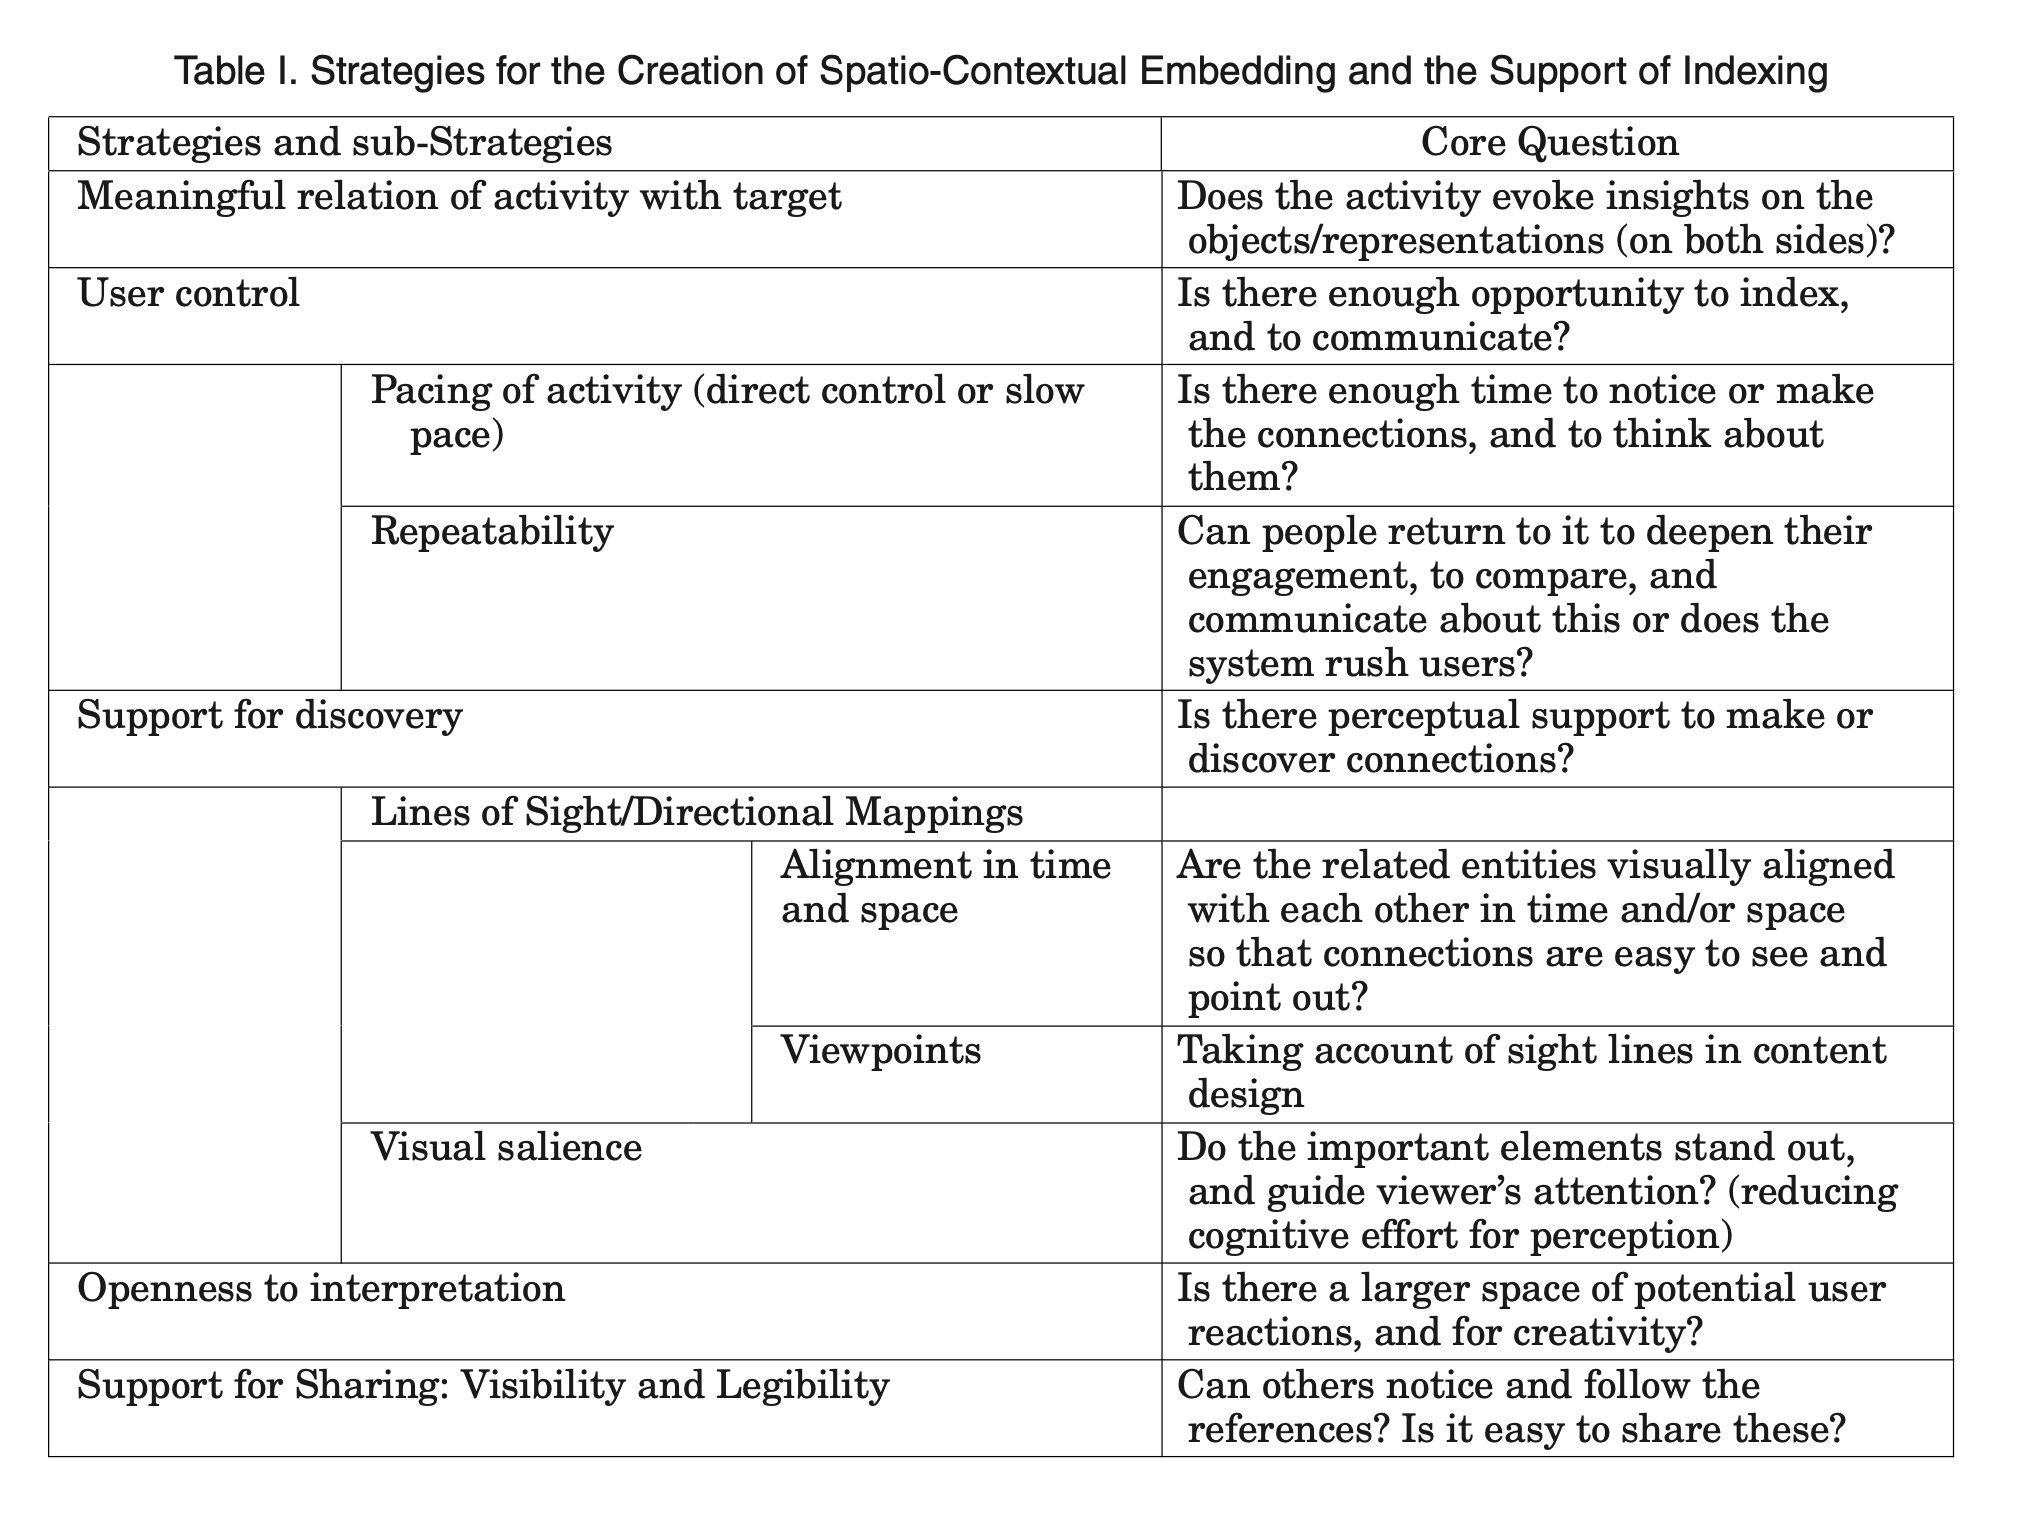
\includegraphics[width=12.5cm]{pictures/strategies.png}
\caption{Sense-making strategies}
\autocite[p. 35]{hornecker_to-and-fro_2016}
\end{figure}